\documentclass{article}

% if you need to pass options to natbib, use, e.g.:
%     \PassOptionsToPackage{numbers, compress}{natbib}
% before loading neurips_2020

% ready for submission
% \usepackage{neurips_2020}

% to compile a preprint version, e.g., for submission to arXiv, add add the
% [preprint] option:
\usepackage[preprint]{neurips_2020}

% to compile a camera-ready version, add the [final] option, e.g.:
%     \usepackage[final]{neurips_2020}

% to avoid loading the natbib package, add option nonatbib:
%    \usepackage[nonatbib]{neurips_2020}

\usepackage[utf8]{inputenc} % allow utf-8 input
\usepackage[T1]{fontenc}    % use 8-bit T1 fonts
\usepackage{hyperref}       % hyperlinks
\usepackage{url}            % simple URL typesetting
\usepackage{booktabs}       % professional-quality tables
\usepackage{amsfonts}       % blackboard math symbols
\usepackage{nicefrac}       % compact symbols for 1/2, etc.
\usepackage{microtype}      % microtypography
\usepackage{graphicx}
\usepackage{float}
\restylefloat{table}
\usepackage{array}
\newcolumntype{L}{>{\centering\arraybackslash}m{3cm}}

\title{Formatting Instructions For NeurIPS 2020}

% The \author macro works with any number of authors. There are two commands
% used to separate the names and addresses of multiple authors: \And and \AND.
%
% Using \And between authors leaves it to LaTeX to determine where to break the
% lines. Using \AND forces a line break at that point. So, if LaTeX puts 3 of 4
% authors names on the first line, and the last on the second line, try using
% \AND instead of \And before the third author name.

\title{Understanding Presidential Speeches\\ and Executive Orders through Natural Language Processing\\
	\large Computational Content Analysis}

\author{Lily Grier \\
	\texttt{lilygrier@uchicago.edu}  \\
	The University of Chicago
	\AND
	Linh Dinh\\
	\texttt{ldinh@uchicago.edu} \\
    The University of Chicago\\
	\AND
	Roberto Barroso-Luque\\
	\texttt{barrosoluquer@uchicago.edu} \\
	The University of Chicago\\}

\begin{document}
\maketitle

\begin{abstract}{
		Our study explores the semantic relationship between presidential speeches and executive orders. Specifically, we are interested in the topics that emerge in speeches and orders, how word use changes over time, and whether there are semantic distinctions between the Republican and Democratic parties. We examine executive orders from the start of Bill Clinton’s presidency up until March 2021 and speeches ranging from Lyndon B. Johnson’s time in office to the beginning of Joe Biden’s presidency. We employ natural language processing techniques such as word frequency analysis, dependency parsing, k-means clustering, topic modeling with Latent Dirichlet Allocation (LDA), word embeddings, and doc2vec. We found that the number of unique words used by each president was mainly a function of how many speeches they gave and the average sentence depth produced by dependency parsing of speeches ranged from 2-6. The distribution of sentiment of presidential speeches is correlated with the general state of the country during each presidential term, with more negatively valence speeches occurring in presidencies overlapping with war or national crisis. We found that k-means clustering was able to distinguish speeches from orders with high accuracy. We performed topic modeling on the two corpuses using a grid search of LDA models. The relationship between topics of executive orders and of speeches varies based on the president: Barack Obama and George W. Bush appear to exhibit the most consistency between speeches and orders. As expected, executive orders exhibit higher degrees of cosine similarity to one another than do presidential speeches, which have more variation. Word and document embeddings revealed partisan differences in conventionally “divisive” topics such as immigration and climate change. Looking at these embeddings over time reveals major shifts at the start of the Trump presidency as well as the start of the COVID-19 pandemic. Our work extends previous analyses of presidential rhetoric by exploring the relationship between communication and tangible political action. This work aligns with the distributional hypothesis of language, which suggests that words that occur in similar contexts have similar meanings and that differences in linguistic form connote differences in meaning. 
	}
\end{abstract}

\newpage
\section{Introduction and Background}{
We are studying how the executive branch of government communicates its goals, purposes and actions with the public, and how it attempts to realize these goals through executive orders. Furthermore, we are investigating the dynamics between various occupants of the oval office and how their unique use of language, party affiliation, and time in office differentiate them. We believe combining an analysis of executive orders and presidential speeches will illuminate the ways that public rhetoric and policy interact. We will see how issue framings translate to concrete policy decisions. Our analysis is limited in that we are only using executive orders to look at policy, while a substantive degree of policy change occurs through legislation passed through the House and Senate.

Grimmer and Stewart (2013) argue that automated text analysis has great potential for extracting insight from large bodies of political text. They argue, “If political scientists can effectively use large collections of text in their inferences, then many substantively important questions are likely to be answered” (29). They caution that the tools used should be specific to the problems at hand, and results produced should be measured against hand-coded comparisons or expert knowledge of relevant concepts. The authors warn, “Applying any one of the methods described here without careful thought will likely lead to few answers and a great deal of frustration” (29). Because our study focuses mainly on unsupervised learning techniques, we will cautiously evaluate the validity of our results and interrogate processes that may have biased our models’ outputs. 

Several previous studies have applied natural language processing techniques to public-facing political rhetoric. Rule, Cointet, and Bearman (2015) examined changes in political discourse from 1790 to 2014 by looking at word co-occurrences of words in State of the Union addresses. They used these co-occurrences to evaluate how ways of talking about certain topics changed over time. Their strategy leverages network clustering to “track the continuity, discontinuity, and relations between categories across time” (Rule et al., 2015). Though the texts in their corpus spanned as far back as the Civil war, they found the political discourse from this time period was transient and that the language of modern politics that persisted into the future did not emerge until World War I. The discursive categories they found included land, production, domestic policy, foreign policy, crime, political economy, navy, statecraft, and immigration.

Savoy (2017) used natural language processing techniques to analyze the style and rhetoric of candidates in the 2016 US presidential primary elections. The author used transcripts from televised debates and looked at the sentence complexity and vocabulary exhibited by each of the candidates. The study found that Donald Trump’s linguistic style diverged in that he used short, simple sentences with a smaller vocabulary size than the other candidates. Ted Cruz was found to use the most descriptive rhetoric and talk about specific people, organizations, and policies more than abstract ideals. Savoy (2017) also employed a term-frequency inverse-document frequency analysis to identify the most distinct words for each candidate. Topical clustering indicated that candidates from the same political party were more likely to talk about the same topics. We believe these methodologies, particularly dependency parsing and word-frequency counts, can help us glean a better understanding of presidential communication styles.

Even before the advent of computational linguistic analysis, scholars have regarded presidential speech as an important facet of American society. Mass media has made the president regularly on people’s radar: whether through news articles and radio segments on his behavior or through direct communication such as televised speeches, press conferences, and social media posts. In a discussion of the prominent role of public communication in the American presidency, Stuckey (2010) claims, “...we do not do nearly enough work that analyzes the connections between the exercise of presidential power and the exercise of presidential rhetoric. Thus, we bring into the picture one of the main ways through which presidents exert power: executive orders. We believe analyzing the semantic relationships between the ways in which presidents communicate to the public and the tangible policies they enact will challenge existing assumptions about the function of the American presidency. 

Executive orders are issued by the president and manage the operations of the federal government. They have the force of law, do not require Congressional approval, and can only be overturned by future executive orders. Executive orders follow a rigid structure. They begin with a heading, title, and introduction. The introduction starts along the lines of “by the authority vested in me as President by the Constitution and laws of the United States of America” and proceeds to detail the motivation behind and context of the order (American Bar Association, 2021). The body of the order is broken into sections and subsections that list the action steps required to carry out the order, the directives for further study or evaluation, and who will oversee these initiatives. Executive orders often have the purpose of establishing committees or task forces composed of members of various federal government departments. Given the highly administrative language found within executive orders, we anticipate that it will be challenging to extract meaningful information from them through merely examining word frequencies and co-occurrences. We will explore techniques better suited to corpuses of highly similar documents and attempt to parse out meaning.

We plan to conduct an exploration of the semantic relationship between US presidential speeches and executive orders. Specifically, we are interested in how the issues a president discusses in their speeches map onto the executive actions they take. We plan to examine two corpuses: a corpus of presidential speeches (from Kennedy to Biden) and a corpus of executive summaries (from Clinton to Biden). We choose to consider the role of the president here and not other political actors because we believe the president has great influence over public perception of policy issues. Further, in recent decades, executive orders have become a more mainstream way for a president to assert their power. It is not uncommon for there to be back-and-forths between successive presidents of alternate parties striking, then reinstating, then striking, then reinstating a particular order. We are interested in examining these interplays, and in looking at how presidents frame and justify the actions they take to the public. A question we have is whether presidents from different parties who focus on similar policy issues might frame those issues in different ways.

This exploration could reveal how the prominence of certain policy issues have evolved over time. In thinking about today’s policy issues, it is important to understand how those issues rose in pertinence. Our study will shed further light on the interplay between public attention and a president’s actions. It may be the case that certain issues garner public support and then the president acts on those issues, or it could be that presidents speak on issues politically important to them, and then the public reacts to those issues, shaping the next president’s actions. This type of analysis can also help us better understand the legacies of our presidents. For example, Obama is known for the Affordable Care Act, but it may also be the case that he reflected the American public’s concerns around climate change in his speeches and actions. Seeing the ebb and flow of policy prominence could help us understand why it’s taken so long to make progress in so many realms and give concrete examples of “one step forward, two steps back” phenomena in our political system. Understanding these patterns is crucial to creating a strategy to effect lasting policy change in the future.

}
\newpage

\section{Methodology}{
\subsection{Data}{We used 2 corpuses for this project: corpus of presidential speeches and corpus of executive orders. The presidential corpus includes 382 presidential speeches from 1963 to 2021 from 12 presidents: Joe Biden, Donald Trump, Barack Obama, George W. Bush, Bill Clinton, George H. W. Bush, Ronald Reagan, Jimmy Carter, Gerald Ford, Richard M. Nixon, Lyndon B. Johnson, and John F. Kennedy. We scraped and downloaded this corpus from https://millercenter.org/the-presidency/presidential-speeches. The executive orders corpus includes 1074 executive orders from 1994 to 2021 from five consecutive presidents: Joe Biden, Donald Trump, Barack Obama, George W. Bush, Bill Clinton. We scraped and downloaded this corpus from https://www.federalregister.gov/presidential-documents/executive-orders.}
\subsection{Word Counts and Dependency Parsing }{In order to understand the lexical idiosyncrasies and differences between presidential speeches, we analyzed individual speeches through finding the most often used words, applying dependency parsing and scoring individual speeches for sentiment. In the coarsest of our analysis we first normalized raw text by tokenizing and stemming individual documents, removing stop words and then counting the number of occurrences for each unique word in each speech. We visualized this analysis by plotting the top ten words used by every president from Lyndon B. Johnson to Joe Biden. Furthermore, we made use of dependency parsing, a text mining technique to capture linguistic dependencies from text. Such methods tag different words in a sentence based on their relationships to other words and the grammatical structure of individual sentences. Dependency parsing gives insights into the dynamic relationship between the different parts of a sentence while also allowing the researcher to understand the complexity of sentences. By using a recursive algorithm, we then navigated all sentences by interpreting them as dependency trees. This recursive analysis allowed us to get the maximum depth of individual sentences, in this paper we interpret dependency depth as language complexity as sentences with more node-levels tend to be syntactically more complex. We then analyzed the minimum, average and maximum sentence depth for all presidents to understand their syntactic style in speeches. 
}

\subsection{Sentiment}{We made use of sentiment analysis, a natural language processing technique that allows for the systematic identification of affective valence across language to quantify the relative valence of individual speeches across and between presidents.  In addition, we made use of sentiment analysis, in conjunction with word embeddings, to understand the relative direction of emotion shown by presidents towards specific policy and legislative problems. It is important to note that in our analysis, as is common in the natural language processing literature, sentiment scores can range between -1 to 1 with negative values denoting detrimental sentiment while positive values signal optimistic sentiment.  
}

\subsection{K-Means Clustering}{To explore the semantic differences and similarities between presidential speeches and executive orders, we applied clustering methods to these corpuses.The raw text from each document (e.g., a presidential speech, an executive order) was vectorized using sklearn TfidfVectorizer. Afterwards, the standard K-Means algorithm was applied to the vectorized texts of all documents. The default sklearn hyperparameters other than the number of clusters were used. And, we used grid search with a number of clusters {2,3,4} for each of three specifications of data: presidential speeches and executive orders combined, presidential speeches only, and executive orders only. The clustering results (number of clusters) with the most reasonable Silhouette Analysis and Principal Component Analysis (2 components visualized) results were reported in the Results section below. Additionally, for the experiment where we combined presidential speeches and executive orders, we know in advance the “true” number of clusters; thus, we also evaluated and reported on a few K-Means accuracy metrics such as Homogeneity, Completeness, V-measure, and Adjusted Rand Score.
}

\subsection{Topic Modelling and Latent Dirichlet Allocation}{To explore how words clustered together in semantic space, we performed topic modeling on both the executive orders and presidential speeches corpuses. After some preliminary cleaning, we tokenized and normalized our text and applied Latent Dirichlet Allocation (LDA). LDA is a machine learning method that attempts to extract meaningful topics from a set of documents based on the distribution of words within those documents. LDA starts off by randomly assigning each word in a document to a topic according to a pre-specified number of topics. It then uses the probability distribution of topics across each document as well as the probability distribution of words across topics to iteratively change the topics assigned to each word. 
Because k-means clustering suggested executive orders and presidential speeches are semantically distinct, which aligns with the more technical nature of executive orders compared to the persuasive aims of presidential speeches, we chose to analyze these two categories of documents as two separate corpuses. 

Preliminary exploration with the executive orders corpus raised the concern that procedural words were creating non-meaningful topics. For example, we had a topic consisting of “shall,” “agency,” “hereof,” and “presidential,” which do not reveal anything about the policy domain in which an executive order lies. To guard against this, we filtered out words common to executive orders that may not be filtered out by the tf-idf cutoff determined by the gensim model. These words included “department,” “shall,” “order,” “federal,” “law,” “president,” “act,” “secretary,” “amendment,” “amend,” “state,” “executive,” “agency,” and “section.” This preliminary step allowed for marginally more meaningful topics found through LDA, though there is certainly room for improvement in effectively filtering out non-meaningful words.
 
For each of our two corpuses, we performed a grid search to find the optimal LDA model specification. As LDA requires the number of topics to be specified in advance, we tried models with 4, 6, 8, 10, 15, and 20 topics. We also varied the range of alpha and beta, trying 0.6, 0.8, and 1.0 for each. Alpha is a hyperparameter which represents topic density. Higher alpha values mean documents will be composed of a greater number of topics. Beta controls the topic-word density. An LDA model with a higher value of beta will produce topics with more similar words to each other. We ranked models based on their coherence scores and performed further analysis on the best-performing model specification from each corpus. The results of the grid searches for each corpus are depicted in Table 1 and 2. 
	
\begin{table}[H]
	\caption{Optimization of LDA Hyper-Parameters through Grid Search: Speeches}
	\centering
	\begin{tabular}{llll}
		\toprule
		\midrule
		Alpha  & Beta & num-topics & coherence-score\\
		\midrule
		\midrule
		.6 & .6 & 10 & .432312   \\
		\midrule
		1 & .8 & 10 & .37757     \\
		\midrule
		asymmetric & .4 & 10 & .37757  \\
		\midrule
		asymmetric & .8 & 15 & .37568  \\
		\midrule 
		.2 & .6 & 15 & .37114    \\
		\midrule 
		... & ... & ... & ...    \\
		\midrule 
		.2 & symmetric & 2 & .2598    \\
		\midrule 
		.4 & 1 & 2 & .25625   \\
		\midrule 
		.6 & .2 & 2 & .2538   \\
		\bottomrule
	\end{tabular}
\end{table}

\begin{table}[H]
	\caption{Optimization of LDA Hyper-Parameters through Grid Search: Executive orders}
	\centering
	\begin{tabular}{llll}
		\toprule
		\midrule
		Alpha  & Beta & num-topics & coherence-score\\
		\midrule
		\midrule
		1 & .8 & 15 & .53   \\
		\midrule
		1 & 1 & 20 & .515     \\
		\midrule
		asymmetric & 1 & 20 & .50  \\
		\midrule
		.6 & .8 & 20 & .492  \\
		\midrule 
		... & ... & ... & ...    \\
		\midrule 
		1 & .8 & 8 & .369    \\
		\midrule 
		1 & .6 & 4 & .365   \\
		\midrule 
		.8 & .6 & 10 & .362  \\
		\bottomrule
	\end{tabular}
\end{table}

}

\subsection{Doc2Vec}{We employed doc2vec on the executive orders corpus to further explore the relationships between documents. Doc2vec is a method that creates numeric representations of documents. We created the following tags as keywords for our documents: “energy,” “environment,” “education,” “labor,” “employment,” “health,” “healthcare,” “defense,” “security,” and “war.” We tagged documents with the keywords they contained, then fed the tagged orders into gensim’s doc2vec model. We also used doc2vec to calculate the cosine similarity between documents and to find documents similar to certain words (e.g., “protect,” “sustainable,” “medicare,” “tax”) as calculated by their vector embeddings, Table 6.}

\subsection{Vector Space Word Embeddings Over Time}{To take into account the semantic changes over time of presidential speeches and executive orders, we looked at the word embeddings of selected focal words by year for the period between 2000 and 2020. The raw text from each document (e.g., a presidential speech, an executive order) was word tokenized and normalized using the word-tokenize and sent-tokenize methods of the lucem-illud package. The sentence structure of each text was retained because it is needed for Gensim Word2Vec’s “continuous bag of words” method for word embeddings. Each unique word in the corpus vocabulary was vectorized using Word2Vec’s “continuous bag of words” - a neural network model on sequences of texts. 
	
In order to identify the semantic changes overtime of focal words relevant to our project, which are “president,” “regulation,” “economy,” “health,” “energy,” “equity,” we needed to analyze the word vector embeddings of these focal words in their semantic space over time. Thus, we first generated one word vector embeddings model for each year using all the tokenized corpus (of both presidential speeches and executive orders) in that year. We chose to combine both presidential speeches and executive orders into 1 single corpus for this analysis because our hypothesis was that the semantic variations can occur in both corpus. Additionally, combining corpuses also allowed us a wider vocabulary of common words (of all years) to investigate. Given that our corpuses were small in size, we realized that a lot of the words (topics) of our interests, which admittedly are more recent “hot” topics, were not present in one or both of our corpuses until very recent years.
	
Afterwards, we aligned the dimensions of the word vector embeddings for all words in the vocabulary that are common in all years. Finally, for each focal word, we calculated the cosine similarities of the vector embeddings between years and visualized them (more specifically, we visualized 1 - cosine similarity) in a heatmap. For this analysis, we restricted the time period to the last 20 years (2000-2020) due to the fact that some of our focal words did not appear until more recent years. 
}
\newpage

\section{Results}{	
\subsection{Word Counts, Dependency Parsing and Sentiment}{To gain a coarse understanding of presidential rhetoric style we counted the number of unique words by each president (Fig 1a). In order to give context, we also counted the number of speeches by each president present in our corpus. In general it seems that the number of unique words is mostly a function of the number of speeches given by a president. For example while Joseph R. Biden is by far the president with the lowest number of unique words used, he is also the president with the smallest number of speeches present in our corpus (just 1). Conversely, Lyndon B Johnson who used more than 11,000 unique words across his speeches did so throughout 70 speeches. Nonetheless, it is worth nothing that both Reagan and Obama, often the most celebrated presidents of their respective parties, made use of more than 12,000 and 11,000 unique words, respectively, during many less speeches than Johnson. 

Our word count analysis, surprisingly, showed that despite party affiliation or era, most presidents seem to use a similar set of ten top words by raw count (Fig 1b). Staple speech words such as america, nation, democracy, united, etc are used frequently by all presidents of both parties. Such regularity, however, does not hold for the sentence complexity across presidents speeches (Fig 1c).  While the average sentence depth of most presidents ranges between 2 and 5 levels, maximum depth has high variance. In the lower end of the spectrum, presidents such as Donald Trump and George W. Bush makes limited use of complicated sentences reaching a maximum of 12 or less in dependency depth. In contrast, president Obama, Clinton, George H.W. Bush and Ford reach a maximum dependency depth of more than 16 levels each. Such differences in sentence complexity illustrates the idiosyncratic style of individual presidents.

In terms of relative valence in presidential speeches (Fig 1d) we see that, in general, presidents tend to be upbeat in their speeches with a vast majority of speeches in our corpus scoring the maximum possible value of 1. Notably, it was republican presidents Donald Trump and George W. Bush who striked a pessimistic tone more often than any other president with each having more than 5 speeches with negative sentiment scores. This result is consistent with the political punditry accounts of both presidents presenting a more cynical and fatalistic world outlook than their counterparts.
}
\newpage
\begin{figure}[H]
	\center{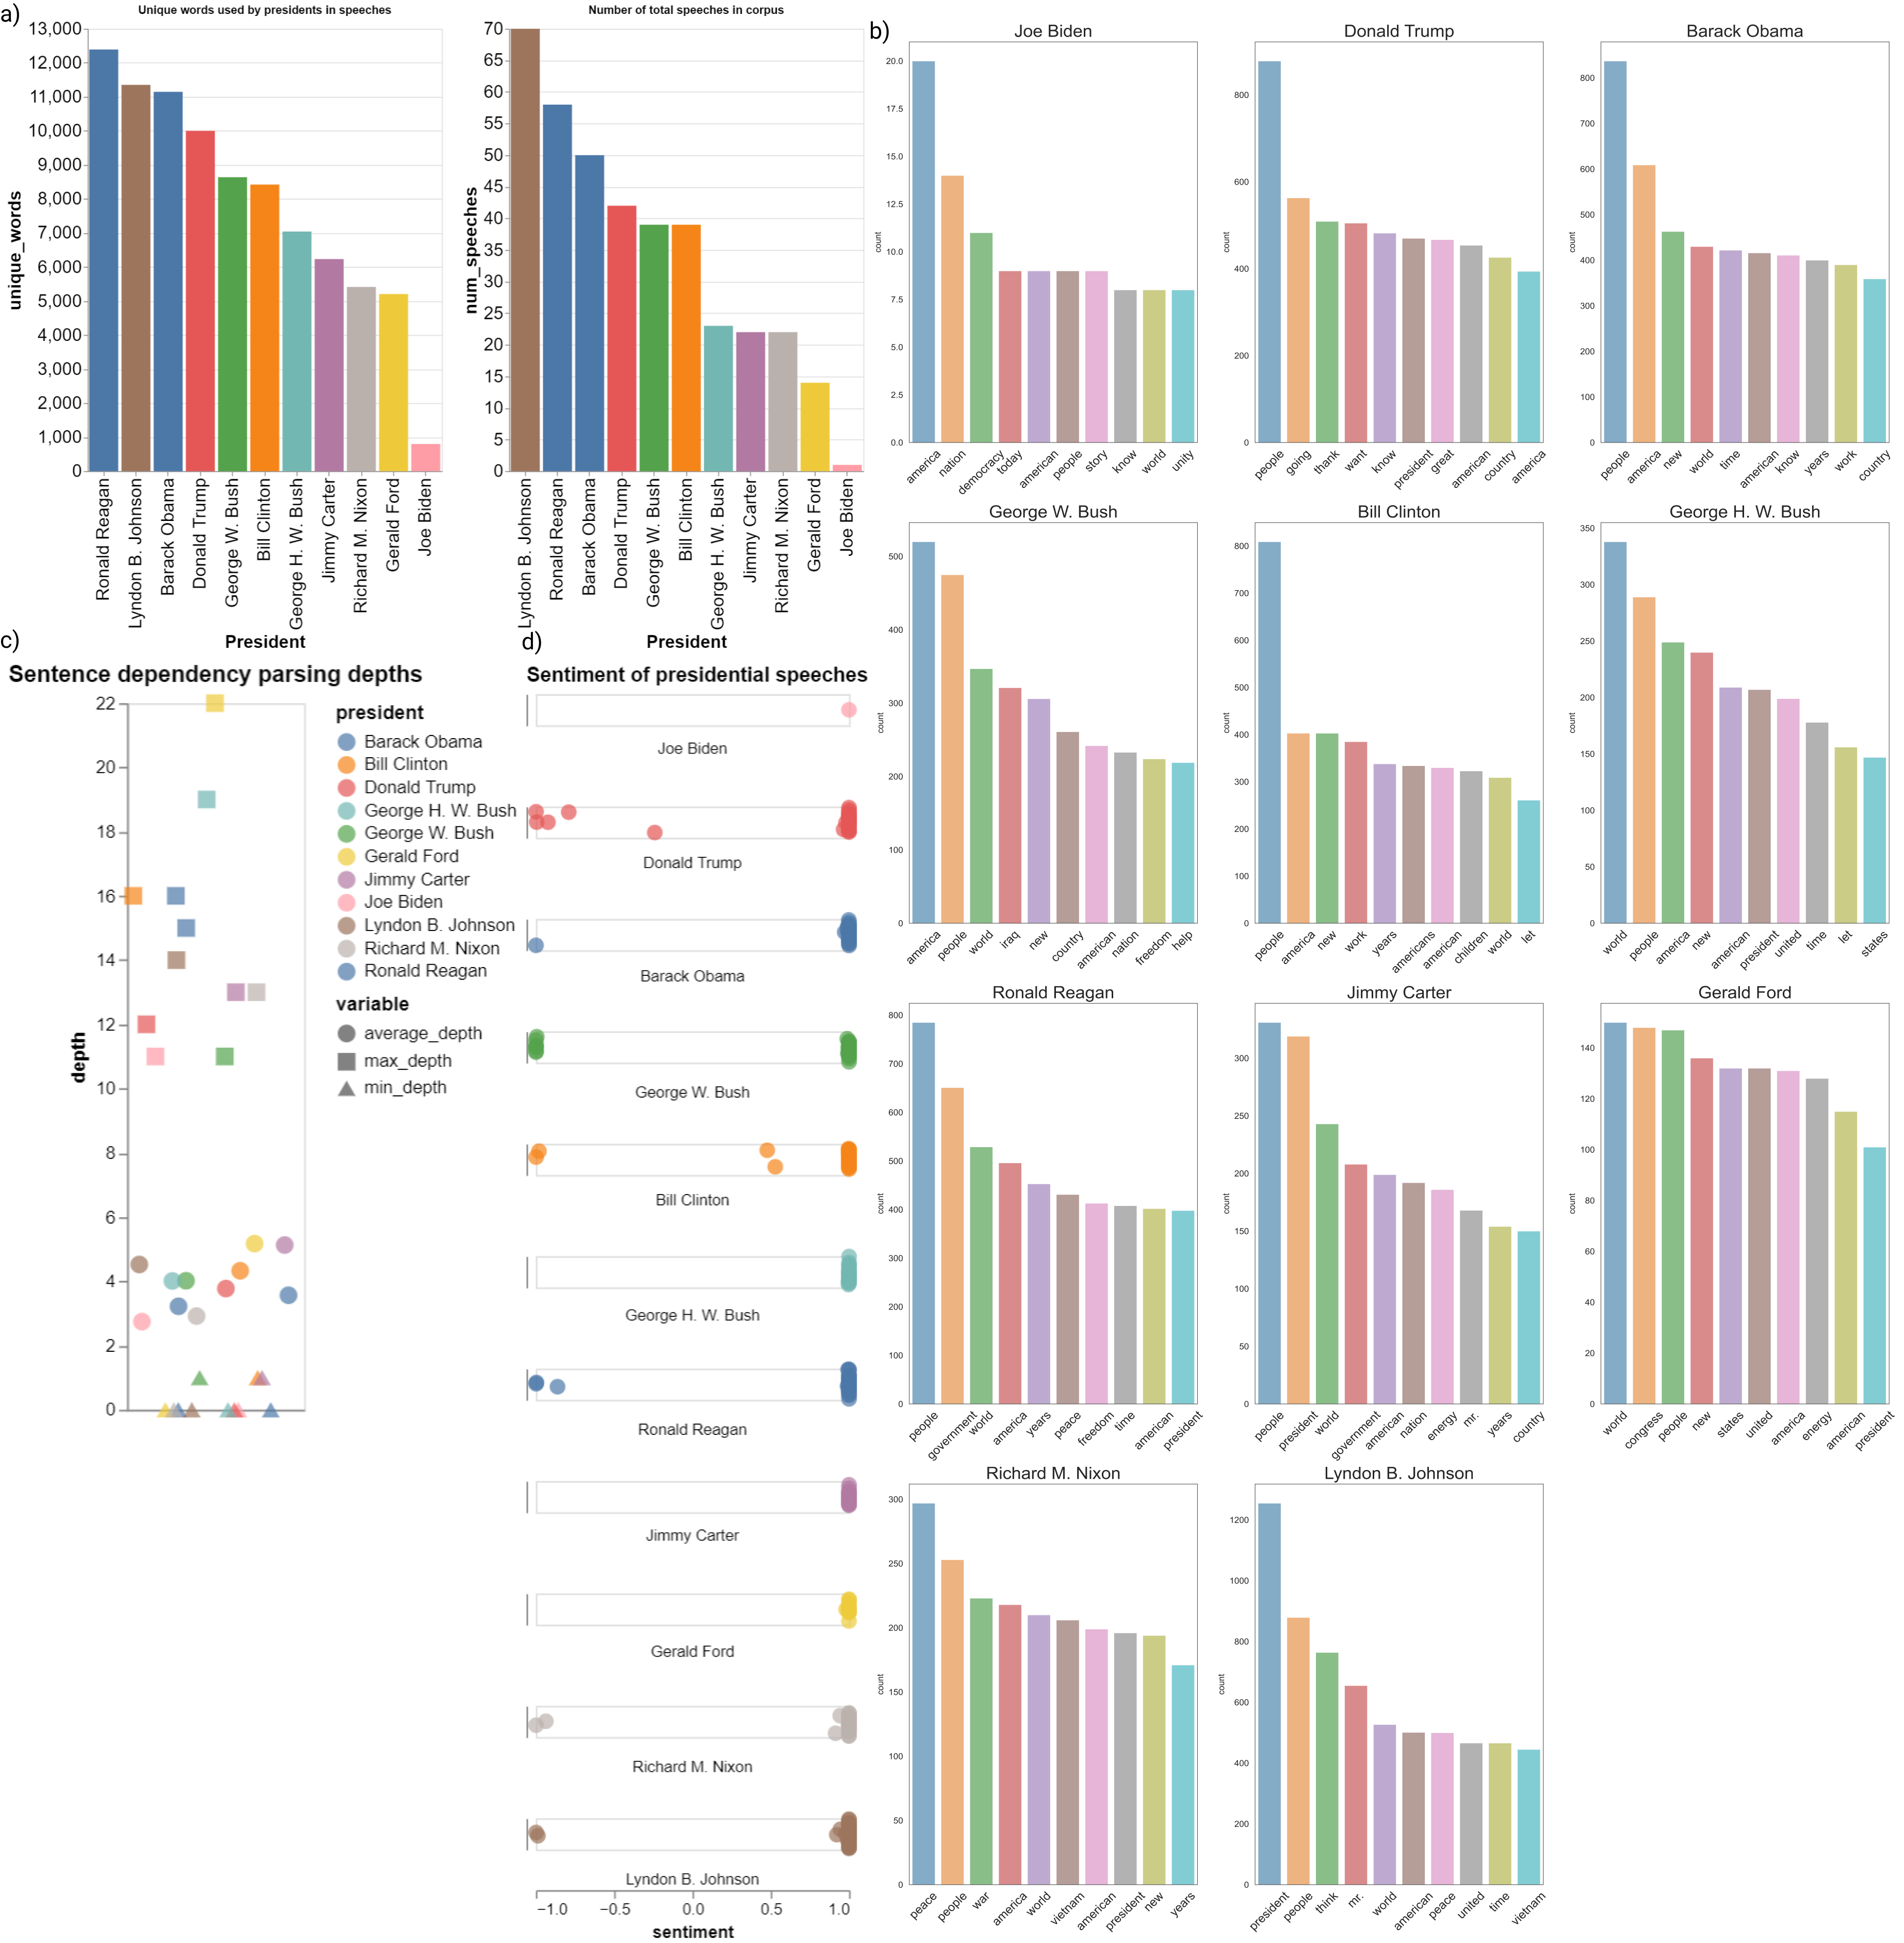
\includegraphics[width=\textwidth]
		{figures/speechesstylepresident.png}}
	\caption{\label{fig:my-label1} Analysis of Presidential Speeches}
\end{figure}
}
\newpage
\subsection{K-Means Clustering}{After investigating the presidential rhetoric style using the presidential speeches corpus, we wanted to examine the semantic distance, if any, between this corpus and the executive orders corpus, as well as seeking higher level patterns in each corpus through clustering techniques. For the data that combined presidential speeches and executive orders, based on Silhouette Analysis, the best number of clusters was 2, which also correctly distinguished between presidential speeches and executive orders as seen in by plotting the 2-first principal components (Figure 2,  top left and right figures). Since we have the “true” clusters in this experiment, we also looked at a few K-Means accuracy metrics, which were all very high and indicated that the K-Means algorithm worked very well with this classification task (i.e., identifying presidential speeches vs. executive orders). The Homogeneity is 0.962, Completeness is 0.968, V-measure is 0.965, and Adjusted Rand Score is 0.986. This result also suggested that the semantic characteristics of presidential speeches are very different from that of executive orders and vice versa.

For the data that contained only presidential speeches or only executive orders, based on Silhouette Analysis, the best number of clusters were also 2 for both datasets. The Principal Component Analysis (2 components) plots also looked reasonable (the bottom left and right figures). We do not have the “true” clusters in these 2 experiments; thus, we could not look at any K-Means accuracy metrics as before. However, the semantic separations within each corpus (i.e., presidential speeches alone and executive orders alone) were investigated with topic modeling and the results were presented in the following sections.

\begin{figure}[H]
	\center{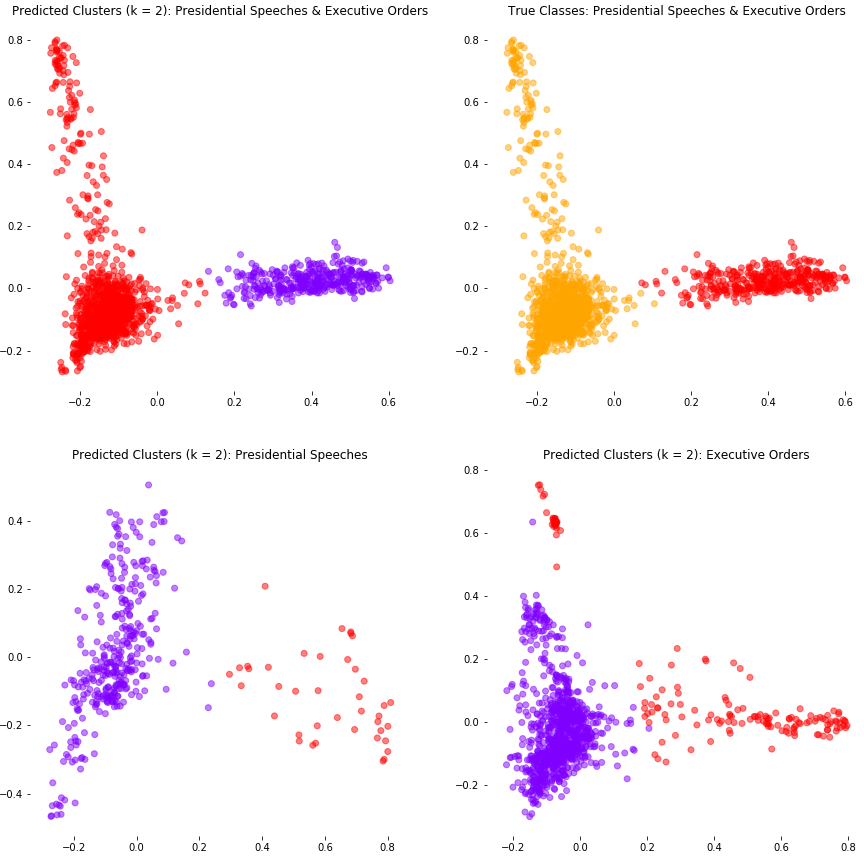
\includegraphics[scale=0.4]
		{figures/clusters.png}}
	\caption{\label{fig:my-label2} K-Means through PCA, Speeches and Executive Orders}
\end{figure}
}
\begin{figure}[H]
	\center{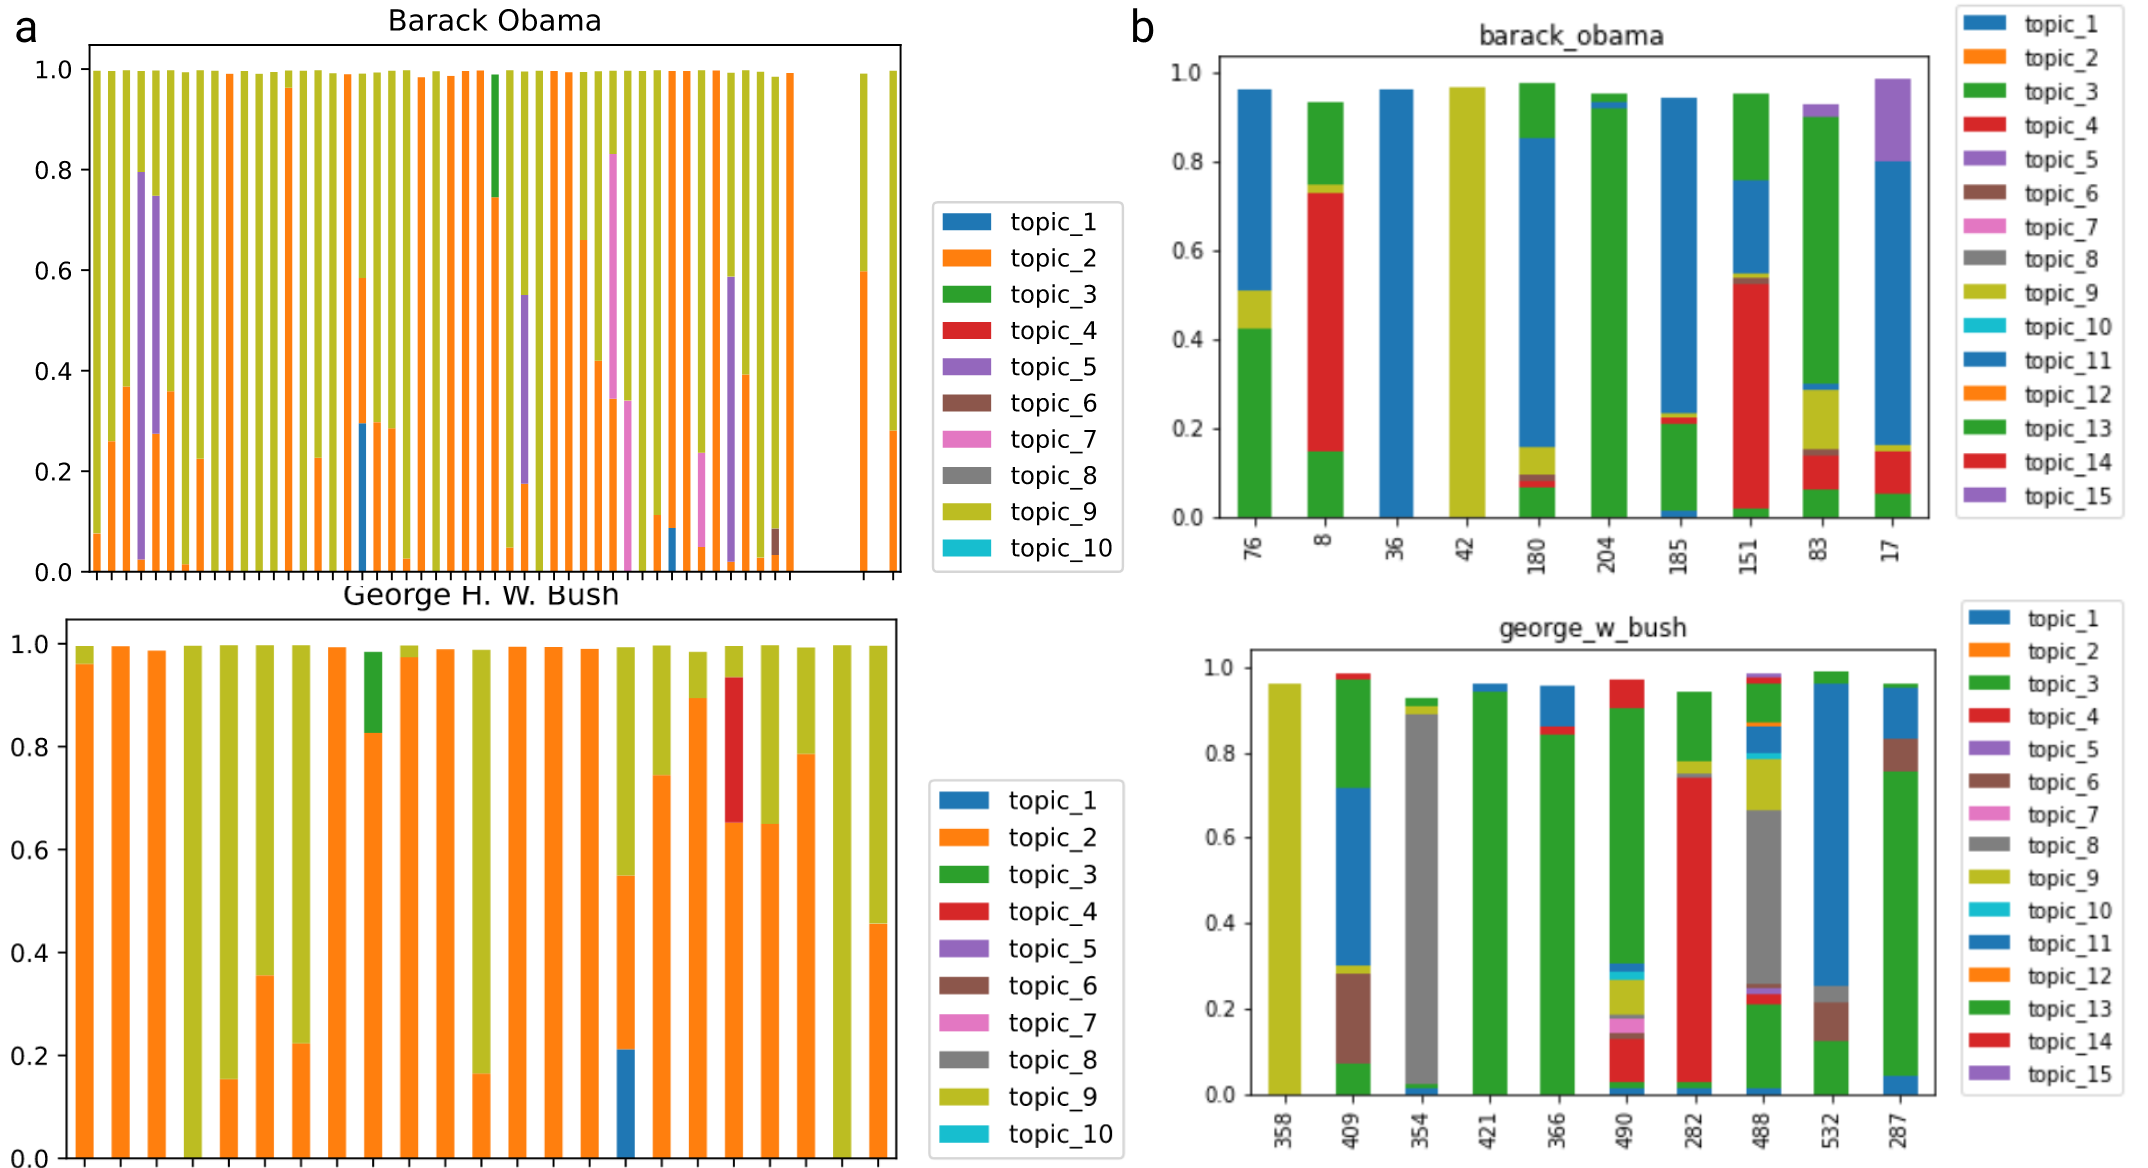
\includegraphics[scale=0.7]
		{figures/Documenttopics.png}}
	\caption{\label{fig:my-label3} Distribution of topics in presidential speeches}
\end{figure}
\subsection{Topic Modeling and Latent Dirichlet Allocation}{
While K-Means clustering provided some high level intuition about the patterns of our text data, especially in separating presidential speeches and executive orders, it could not provide deeper insights into how to identify and interpret the nuance patterns within each corpus. Therefore, after K-Means clustering, we separately performed LDA on our presidential speeches and executive orders corpuses.

Presidential Speeches LDA \\
Our optimal LDA model for the presidential speeches corpus, with a coherence score of 0.432, had 10 topics, an alpha value of 0.6 and a beta value of 0.6. The top 10 words for each cluster are shown in supplementary figure 2. 
We assigned each topic an informal label based on its most prominent words and our knowledge of common topics within presidential speeches in Table 3.
When we looked at the breakdown of topics across individual speeches, we saw that each president in our corpus mainly spoke about topic 1 (welfare and aid) and topic 8 (diversity and inclusion) in his first speech as president, which is presumably the inaugural address. This makes sense, as these topics are about helping those in need and embracing the American public and can be framed in party-neutral ways. Inaugural speeches generally focus on abstract American ideals and less on concrete policies, talking about broad topics such as peace and the strength of the American people rather than war or health insurance.Visualizing the breakdown of topics by president provides insight into variations in policy focuses. Below (Figure 3) we have topic distributions for Barack Obama and George W. Bush. Obama’s speeches cluster around topic 9, the people’s president, which Bush’s speeches center around topic 2, America and the world, which makes sense as Bush’s presidency is characterized by the wars in Iraq and Afghanistan and growing fears around national security following the 9/11 attacks. We also see health insurance as a prominent topic in Obama’s speeches, which aligns with the narrative of the passing of the Affordable Care Act as Obama’s most notable accomplishment.  

\begin{table}[H]
	\caption{Informal Labels for Optimized LDA Speeches Model}
	\centering
	\begin{tabular}{ll}
		\toprule
		\midrule
		Topic id  & Topic name \\
		\midrule
		\midrule
		1 & Welfare and aid \\
		\midrule
		2 & America and the world \\
		\midrule
		3 & Foreign wars \\
		\midrule
		4 & Great power rivalry \\
		\midrule
		5 & Celebrations \\
		\midrule
		6 & Supreme Court \\
		\midrule
		7 & Health insurance \\
		\midrule
		8 & Diversity and inclusion \\
		\midrule
		9 & The people’s president \\
		\midrule
		10 & NATO and proxy wars \\
		\bottomrule
	\end{tabular}
\end{table}

Executive Orders LDA \\
The optimal LDA model for the executive orders corpus, with a coherence score of 0.542, had 20 topics, an alpha value of 0.8, and a beta value of 1. The topics with their informal names and top keywords are in Table 4. 

\begin{table}[H]
	\caption{Informal Labels for Optimized LDA Executive Orders Model}
	\centering
	\begin{tabular}{lll}
		\toprule
		\midrule
		Topic id  & Topic name & Salient Words \\
		\midrule
		\midrule
		1 & Military procedures & Follow, court, martial, military, punishment \\
		\midrule
		2 & Health insurance & Health, care medicare, affordable, coverage \\
		\midrule
		3 & Payment systems & Schedule, pay, rate, service, adjustment \\
		\midrule
		4 & International crime & Turkmenistan, interpol, combatant, vested  \\
		\midrule
		5 & National security/intelligence & Security, information, national, intelligence, homeland \\
		\midrule
		6 & Census & Census, race, population, status, sex, apportionment\\
		\midrule
		7 & Crisis & Pursuant, emergency, foreign, prohibit, block\\
		\midrule
		8 & Life Sciences/Biology & Genetic, mutation, diagnose, metabolic, chromosomal\\
		\midrule
		9 & Monuments & Statue, monument, national, hero, Washington, memorial\\
		\midrule
		10 & International crime & Turkmenistan, vested, interpol, combatant\\
		\midrule
		11 & Governmental bureaucracy & Committee, register, commission, member, advisory\\
		\midrule
		12 & Internet regulation & Platform, online, speech, restrict, deceptive, ftc, twitter\\
		\midrule
		13 & Space & Space, command, nuclear, weather, exploration, moon, nasa\\
		\midrule
		14 & Public health & Agency, health, public, covid, community, program\\
		\midrule
		15 & Foreign diplomacy & Immunity, international, binational, israel, european\\
		\midrule
		16 & Labor issues & Board, dispute, railroad, employee, company, union, represent\\
		\midrule
		17 & Military honors & Medal, award, arm, navy, guard, coast, terrorism, war, iraq, afghanistan\\
		\midrule
		18 & People in authority & Employee, director, general, title, head, officer\\
		\midrule
		19 & National security & Information, classify, classification, security, national, provide\\
		\midrule
		20 & Energy production & Contractor, energy, facility, use, cost, vehicle, environmental, chemical\\
		\bottomrule
	\end{tabular}
\end{table}

This topic model had some limitations. First, two sets of the topics produced were nearly indistinguishable from one another. Topics 4 and 10 both centered around international crime, while topics 5 and 19 both centered around national security and intelligence. The grid search jumped from 15 to 20 topics, so future research could test topic numbers in between to see if a more optimal topic distribution exists. Further, topics 11 and 18, loosely titled “governmental bureaucracy” and “people in authority,” respectively, are not very informative, as they mostly contain procedural words (e.g., “committee,” “member,” “advisory,” “director,” “officer,” etc.). 

Despite its limitations, the topic model does convey some useful insights about our corpus of executive orders. We see major topics of executive orders such as health insurance, scientific research, and foreign diplomacy. Interestingly, healthcare clustered into two distinct topics: one focusing on public health (including COVID-19) and associated infrastructure and the other associated with health insurance. That the model was able to pick up on these contextual nuances speaks to its power in helping us better understand the semantic landscape of executive orders. It makes sense that payments were their own topic, as an order entitled Adjustment of Certain Rates of Pay which modifies the wages of federal employees gets passed almost every single year. 

The topics in this model suggest that executive orders focus more on foreign policy, healthcare, and national priorities such as research than on matters such as labor and regulation of businesses. Perhaps because labor laws vary across state jurisdictions and there is not much tangible policy the executive branch can enact on this front, executive orders don’t hone in on domestic labor and economic policy. We can use these topic models to visualize the topics that different presidents emphasize. 

We coded each order by its dominant topic, then plotted the distribution of dominant topics for each president. Across all presidents, we see our “filler” topics of governmental bureaucracy and people in authority appearing as frequent dominant topics. Future iterations upon this work should try to eliminate these topics through tf-idf filtering or deleting non-meaningful topics and then re-classifying documents into the existing topics. 
Notably, the public health topic and not health insurance was prominent in Obama’s executive orders, though health insurance was a major topic in his speeches. Because the actual passing of the Affordable Care Act occurred through congressional legislation and not through executive orders, it is probable that Obama’s orders made more general declarations about public health than they supported specific insurance policies or healthcare systems. For George W. Bush, we see crisis, national security, and public health emerge as major topics. Bush served as president during major crises such as Hurricane Katrina and the 9/11 attacks and did indeed have many orders aimed toward various mechanisms for homeland security. Though the dataset contains only the first two months of Biden’s presidency, we see the public health topic dominating most of his 37 orders, which fits for a president who came into office during the height of a pandemic.

\begin{figure}[H]
	\center{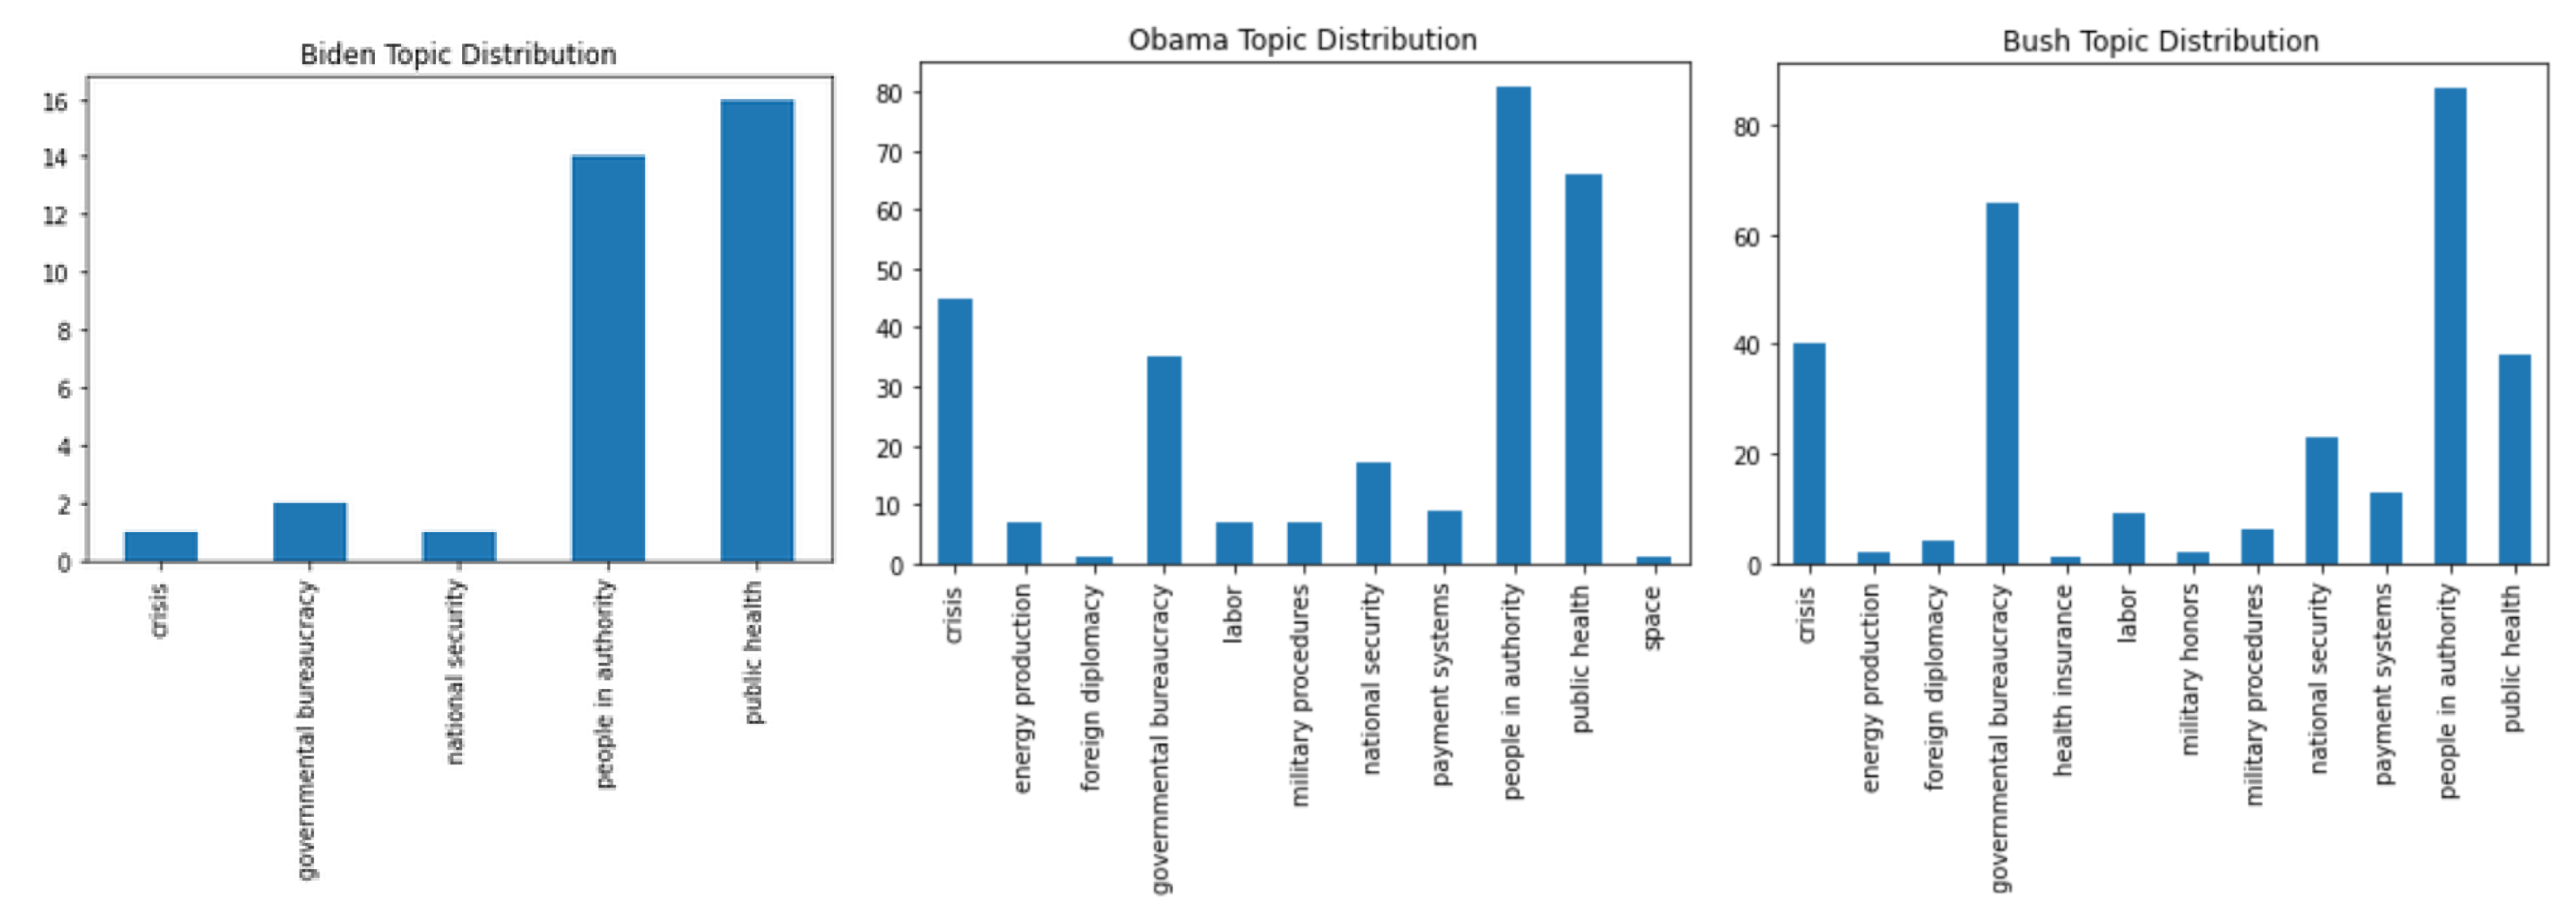
\includegraphics[width=\textwidth]
		{figures/topicdistributions.png}}
	\caption{\label{fig:my-label4} Executive orders LDA Topics distribution}
\end{figure}

\newpage

Comparison of Topic Distribution in Executive Orders and Presidential Speeches \\
The “America and the world” and “the people’s president” topics accounted for most of the presidential speeches, and “governmental bureaucracy” and “people in authority” accounted for most of the executive orders. Because much of the text in our corpuses was classified under these more abstract topics rather than the policy-specific topics, relationships between topic distributions of each president’s topics and speeches were not as clear as we had hoped. However, we can see a few significant patterns when we look beyond these filler topics.

Health insurance emerged as a prominent topic Obama’s speeches, and public health was the dominant topic in a substantial number of his executive orders. Health insurance did not emerge as a topic in our corpus of executive orders, but it is possible that the documents classified as pertaining to public health also pertain to health insurance. It is also possible that Obama produced executive orders that complemented the Affordable Care Act, which was passed as an official law through Congress, and framed these orders in terms of being in service of public health.

The topics in Bush’s speeches were also reflected in his executive orders. Our topic model suggests that Bush’s speeches mostly focused on foreign wars and “America and the world.” The executive orders topic model reveals that Bush’s order centered around crisis and national security. Given 9/11 and the wars in Iraq and Afghanistan during his presidency, it makes sense that Bush would prioritize these matters in his public communications as well as in his substantive policy actions.

A lot of populist language emerged in Trump’s speeches, as reflected in the prominence of “the people’s president” topic. Celebrations, the Supreme Court, and health insurance also appeared as salient topics within Trump’s speeches. His orders mostly centered around “people in authority,” which means they involved many official government offices, committees, and task forces. Public health and crisis were also significant topics in his executive orders. The focus on people in authority is consistent with the narrative of Trump as a president who talks directly about his thoughts and policy goals, and is not afraid to turn to executive orders to turn these thoughts into law. 

We do not see a strong link between the topics that dominate Clinton’s speeches and executive orders. Clinton’s prominent speech topics were “the people’s president,” foreign wars, and NATO and proxy wars. His most prominent executive order topics were governmental bureaucracy, people in authority, and public health. Notably, none of foreign diplomacy, national security, or international crime appeared as salient topics in Clinton’s orders, which is what we would have expected given his speech topics. This might be an artifact of our executive orders topic model lacking the robustness to discern substantive policy topics from legal jargon. It may also suggest a shift in the nature of executive orders following the Clinton presidency, which was the oldest term we included in our analysis. Refining the executive order topic model and performing an analysis on a corpus of executive orders going back further in time could provide valuable insight into the relationships between orders and speeches, as well as how each has evolved over time. 
}


\begin{table}[H]
	\caption{Document-to-word mappings in Executive Orders}
	\centering
	\begin{tabular}{llll}
		\toprule
		\midrule
		Word  & Similarity & Executive Order & President\\
		\midrule
		\midrule
		contractor & .7118 & Combating Race and Sex Stereotyping & Donald Trump \\
		\midrule
		employee & .6772 & Combating Race and Sex Stereotyping & Donald Trump \\
		\midrule
		employment & .67 & Combating Race and Sex Stereotyping & Donald Trump \\
		\midrule
		position & .644 & Combating Race and Sex Stereotyping & Donald Trump \\
		\midrule 
		appointee & .636 & Combating Race and Sex Stereotyping & Donald Trump \\
		\midrule 
		contractor & .7118 & Combating Race and Sex Stereotyping & Donald Trump \\
		\midrule
		attend & .8277 & Establishing Community Solutions Council & Barack Obama \\
		\midrule
		representation & .7807 & Establishing Community Solutions Council & Barack Obama  \\
		\midrule
		partnership & .7804 & Establishing Community Solutions Council & Barack Obama \\
		\midrule 
		diverse & .7768 & Establishing Community Solutions Council & Barack Obama \\
		\midrule 
		patriotic & .767 & Establishing Community Solutions Council & Barack Obama \\
		\midrule
		usrap & .7106 & Programs To Resettle Refugees for the Impact of Climate Change & Joseph Biden \\
		\midrule
		deficiency & .649 & Programs To Resettle Refugees for the Impact of Climate Change & Joseph Biden \\
		\midrule
		aggressive & .647 & Programs To Resettle Refugees for the Impact of Climate Change & Joseph Biden \\
		\midrule
		refugee & .6462 & Programs To Resettle Refugees for the Impact of Climate Change & Joseph Biden \\
		\midrule 
		crucial & .6457 & Programs To Resettle Refugees for the Impact of Climate Change & Joseph Biden \\
		\bottomrule
	\end{tabular}
\end{table}

\subsection{Doc2Vec}{Because LDA results on executive orders provided us with not-so-obvious topics, we wanted to further investigate additional patterns within this corpus leveraging the Doc2Vec model. However, as expected, all orders in our executive order corpus exhibited relatively high cosine similarity, and a simple document-document comparison failed to identify meaningful differences between orders. Because executive orders tend to be largely similar regardless of their content focus and follow a rigid structure, doc2vec may not pick up more nuanced similarities. Attempting to parse out the content of executive orders from their overall structure could be an avenue for future research. 
	
We also used doc2vec to find the most similar words to certain document embeddings, Table 5. Combating Race and Sex Stereotyping, an infamous order enacted by Donald Trump that argued against diversity, equity, and inclusion initiatives that talk about structural racism, exhibited similarity to “contractor,” “employee,” “employment,” “position,” and “appointee.” Interestingly, the main words in this topic don’t have to do with race or gender but rather the workplaces in which these trainings take place. This may be because a greater number of executive orders talk about employees than diversity initiatives, so the model picked up on these procedural elements more. 
	
Obama’s 2016 order, Establishing a Community Solutions Council, mapped onto “attend,” “representation,” “partnership,” “diverse,” and “patriotic.” It called for a council to oversee and support community-based initiatives ranging from workforce training programs to food access to environmental justice. The word mappings here are not surprising, as they refer mostly to the broader goals and motivations of the act rather than the wide-ranging policy areas. 
	
As a third illustrative example of document-to-word mappings, we looked at Biden’s 2021 act entitled Rebuilding and Enhancing Programs to Resettle Refugees and Planning for the Impact of Climate Change Migration. The act mapped onto “usrap” (an acronym for United States Refugee Admissions Program), “deficiency,” “aggressive,” “refugee,” and “crucial.” The words “deficiency,” “aggressive,” and “crucial” do not actually appear in the text of this order, so it is notable that they came up as having similar embeddings. The order emphasizes the need for the United States to increase its capacity for taking in refugees and the heightened urgency of this need given climate change displacing many individuals around the world. Thus, it makes sense that an emphasis on inadequate capacity would link to “deficiency” and stressing the need to enhance our efforts in a timely manner would link to “aggressive” and “crucial.” 

Figure 5 depicts 10 orders selected at random and shows their cosine similarity to each of our 10 keywords. Some of these mappings are more accurate than others. For example, Promoting Beautiful Federal Civic Architecture exhibits puzzling similarity with war and environment. The order establishing a board to investigate labor disputes with the Southeastern Pennsylvania Transportation Authority maps onto labor and employment as expected, but also exhibits strong similarity to security. Thus, there is reason to doubt these mappings are robust enough to classify unlabeled documents. This lack of robustness could be due to executive orders having similar forms and focusing more on specifying administrative procedures rather than on domain-specific policy substance. Future research should seek to better understand the quality of these embeddings, especially for topics such as education and labor, which are less commonly addressed by executive orders.

We also used our doc2vec model to find orders that mapped most strongly onto certain words. For example, we saw that “sustainable” mapped onto orders establishing the Great Lakes Interagency Task Force, managing forests and federal lands, and supporting the use of space resources. Similarly, “tax” mapped onto orders promoting the purchasing of American-made products, encouraging the use of energy efficient devices, making changes to regulation, and supporting the growth of the economy.  Tax also exhibited strong similarity to an order restricting access to abortions, and upon inspection of the order’s text, we found that the order prohibits the use of tax credits to pay for abortions under the Affordable Care Act. 

Doc2vec also proves to be useful for identifying executive orders that map onto combinations of keyword embeddings. For example, adding together the vector embeddings for “land,” “protect,” and “water” fetched orders on protecting and managing forests and trails, reducing wildfire risk, restoring the gulf coast, and recovering space resources. Though this preliminary analysis is not exhaustive, it gives us reason to believe doc2vec could be an effective tool to identify orders that map onto keywords.
}
\begin{table}[H]
	\caption{Document-to-vector results for different keywords}
	\begin{tabular}{|c|c|L}
		\toprule
		\midrule
		Keyword & similarity & Executive order \\
		\midrule
		\midrule 
		sustainable & .778 & \multicolumn{1}{m{8cm}|}{Establishment of Great Lakes Interagency Task Force and Promotion of a Regional Collaboration of National Significance for the Great Lakes}   \\
		\midrule
		sustainable & .7536 & \multicolumn{1}{m{8cm}|}{Encouraging International Support for the Recovery and Use of Space Resources}   \\
		\midrule
		sustainable & .7482 & \multicolumn{1}{m{8cm}|}{Recreational Fisheries}   \\
		\midrule
		sustainable & .7209 & \multicolumn{1}{m{8cm}|}{A Federal Strategy To Ensure Secure and Reliable Supplies of Critical Minerals}   \\
		\midrule
		sustainable & .6889 & \multicolumn{1}{m{8cm}|}{Promoting Active Management of America's Forests, Rangelands, and Other Federal Lands To Improve Conditions and Reduce Wildfire Risk}   \\
		\midrule
		tax & .8164 & \multicolumn{1}{m{8cm}|}{Steps to Increase Competition and Better Inform Consumers and Workers to Support Continued Growth of the American Economy}   \\
		\midrule
		tax & .8144 & \multicolumn{1}{m{8cm}|}{Energy Efficient Standby Power Devices}   \\
		\midrule
		tax & .8017 & \multicolumn{1}{m{8cm}|}{Strengthening Buy-American Preferences for Infrastructure Projects}   \\
		\midrule
		tax & .7889 & \multicolumn{1}{m{8cm}|}{Improving Regulation and Regulatory Review}   \\
		\midrule
		tax & .767 & \multicolumn{1}{m{8cm}|}{Ensuring Enforcement and Implementation of Abortion Restrictions in the Patient Protection and Affordable Care Act}   \\
		\midrule
		land+protect+water & .766 & \multicolumn{1}{m{8cm}|}{Encouraging International Support for the Recovery and Use of Space Resources}   \\
		\midrule
		land+protect+water & .762 & \multicolumn{1}{m{8cm}|}{Promoting Active Management of America's Forests, Rangelands, and Other Federal Lands To Improve Conditions and Reduce Wildfire Risk}   \\
		\midrule
		land+protect+water & .7213 & \multicolumn{1}{m{8cm}|}{Trails for America in the 21st Century}   \\
		\midrule
		land+protect+water & .7213 & \multicolumn{1}{m{8cm}|}{Management and General Public Use of the National Wildlife Refuge System}   \\
		\midrule
		land+protect+water & .619 & \multicolumn{1}{m{8cm}|}{Gulf Coast Ecosystem Restoration}   \\
		\midrule
		\bottomrule
	\end{tabular}
\end{table}

\begin{figure}[H]
	\center{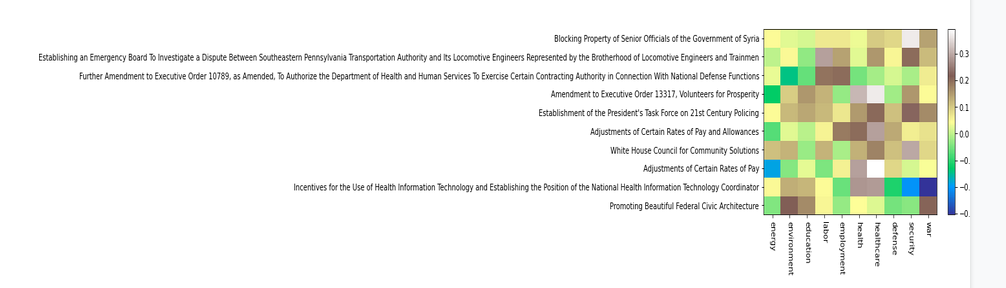
\includegraphics[width=\textwidth]
		{figures/executivewordembedings.png}}
	\caption{\label{fig:my-label9} Cosine Similarity in Executive Orders}
\end{figure}
\subsection{Word Embeddings and Semantic Partisan Difference}{
In addition to using word embeddings to understand the different uses of words by the president, we also sought to analyze the different meanings of words as used by presidents of different parties. By using a vector representation of presidential speeches, we generated two word embedding models by separating our corpus into democratic presidents and republican presidents. We then selected a set of climate-change related words since this topic tends to be a controversial legislative issue. These embeddings illustrate semantic differences between the use of the same word just based on party affiliation. For example when looking at the closest (smallest cosine distance) words to climate, we see that in the democrat's embedding we have words such as suffer, ignore, decay, lesson and realize, while in the republican embedding we have reconciliation, reveal, breakthrough, repression. These different semantic relationships with the word climate exemplify the connotation that politicians give to it. 
Furthermore, as seen in Table 7, by using word embeddings we were able to find the closest words to specific key terms such as the word “fuel”.  For democrats the closest words to “fuel” are natural, pollution, modernize, switch, renewable, etc. While those for republicans are completely, gas, significant, overall, target, shipment, etc.
We then used sentiment scoring to understand the valence presidents of different political parties attribute to these words. While it is no surprise we are able to surface patterns such as republicans having a positive set of words when talking about coal, while democrats are much more neutral. Furthermore, while democrats speak negatively of oil, republicans tend to speak in positive terms about fossil fuel.

\begin{table}[H]
	\caption{Partisan Semantic Word use Difference}
	\centering
	\begin{tabular}{llll}
		\toprule
		\midrule
		Keyword  & Party & closest-words & sentiment\\
		\midrule
		\midrule
		climate & Republican & presence, willingness, refuse, rely  & .296  \\
		\midrule
		climate & Democrat & wall, painful, cripple, urgent, setback & -.273   \\
		\midrule
		coal & Republican & gas, fuel, exploration, accelerate & .452   \\
		\midrule
		coal & Democrat & spur, rapidly, pollution, supply & 0.0   \\
		\midrule 
		oil & Republican & production, massive, large, development & 0.0    \\
		\midrule
		oil & Democrat & half, gross, total, reduce & -.477   \\
		\bottomrule
	\end{tabular}
\end{table}}

\subsection{Vector Space Word Embeddings Over Time}{
Lastly, in addition to looking at the semantic changes between presidents or party affiliations, we could also investigate these changes year by year, thus able to notice if changes occur within a president’s term. 
	
One thing to note was that some of the words (topics) of our interests such as “climate” or “environment” were not present in the yearly corpus of presidential speeches and executive orders until very recent years (i.e., after 2010). Hence, another set of analyses into the appearance and disappearance of words in these 2 corpuses could be interesting; however, the scope of this paper did not address this issue.

As seen from the above figures, a lot of the semantic meaning of our focal words, including “president,” “regulation,” “economy,” and “equity” had a significant change in 2017, which coincided with the inauguration of Donald Trump. This result suggested that, as expected, Donald Trump is quite different from the other presidents, at least in the usage of words and vocabularies in presidential speeches and executive orders in his first year. The significant change of the focal word “equity” in 2017 was particularly intriguing. However, it seems that these changes occurred only in the first year of his term, suggesting that the non-traditional semantic characteristics of a president might only be obvious in the inaugural year. 

Another interesting observation was that there were a lot of big semantic changes in the year 2020, at least among the focal words we chose to look at, which includes “president,” “regulation,” “economy,” “health,” and “equity.” This result seems to suggest that 2020 was indeed a “special” year. We anticipated that the events and sentiments surrounding Covid-19 probably impacted these semantic evolvements. This hypothesis was further corroborated via the fact that the word “health” had a sudden significant change in its semantic embedding in 2020. Before 2020, the word “health” had a relatively stable semantic embedding throughout the past 20 years. Ideally, additional investigations into the potential drivers of these semantic changes could be interesting (such as just simple word counts in case words such as “health” and “equity” appear more often in 2020).

One last observation was how the word “economy” started to fluctuate in its semantic space in 2005, which was slightly before the 2008 financial recession. This suggested that investigating the word vector embeddings of presidential speeches and executive orders somehow was able to anticipate the financial crisis in 2008. Although, further analyses should be done before reaching such a conclusion.
}
\begin{figure}[H]
	\center{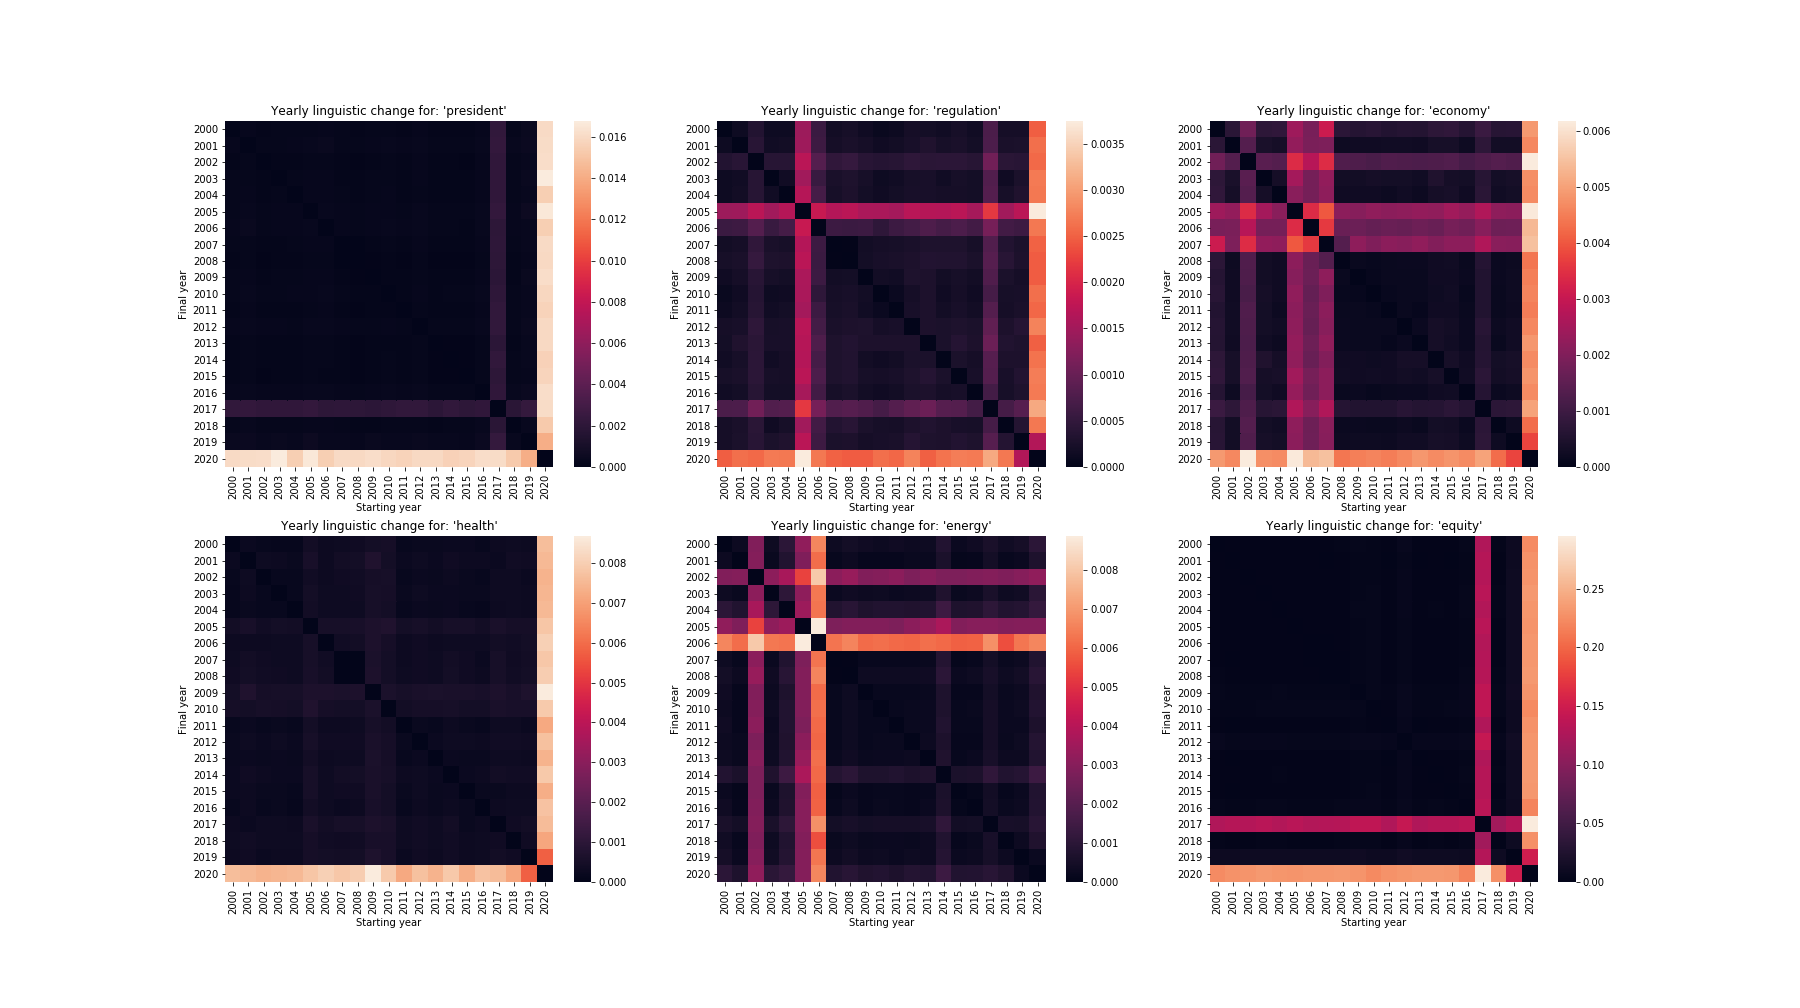
\includegraphics[width=\textwidth]
		{figures/SWEovertime.png}}
	\caption{\label{fig:my-label7} Word Embeddings, visualizing word change use over time}
\end{figure}
}
\newpage
\section{Conclusion, further research and limitations}{
The rapid recent development of computational methods for linguistic analysis has allowed a myriad of fields to investigate what just a few decades ago would have been prohibitively long corpuses. In this research we demonstrate the use of these methods to understand the role of the executive branch in american legislation. Using dependency parsing, clustering, topic modeling and word embeddings we demonstrate the subtle relationship between presidential rhetoric through speeches and executive orders. Dependency parsing, word counts, and sentiment analysis showed the idiosyncratic nature of presidential speeches. The now-ubiquitous k-means clustering algorithm allowed us to semantically distinguish between speeches and clusters without a priori knowledge. Topic modeling using Latent Dirichlet Allocation surfaced the distribution of topics in presidential speeches and executive orders and allowed us to understand legislative priorities among former US presidents. Finally, we captured the linguistic and semantic differences in the use of specific words across time by using vector space word embeddings, while illustrating the high similarity between executive orders. Our analysis adds evidence to the growing literature supporting the principle of contrast as well as the distributional hypothesis of language. That is, in both corpus studied here, words that occur in similar contexts have similar meanings and their differences in linguistic form are accompanied by a difference in meaning.  

Our work makes inferences about relationships between the Democratic and Republican parties in the United States, the role of the American presidency in a democratic society, and the impact presidential speeches and executive orders have on policy changes. Our analysis is limited in that we are only including presidents in our corpus; future work could include other elected officials. It would be interesting to look at House members who draft legislation and the ways they communicate about policy issues (or how Senators vote on issues and the speeches they make to their home states). 

The highly rigid structure of executive orders made it difficult to parse out substantive policy content from specifications of committees and procedures. Topic modeling on this corpus produced a couple of filler topics that consisted of technical jargon and were not useful in semantically distinguishing documents. While we filtered out words that we noticed appear frequently in executive orders and do not pertain to specific policies, a more systematic approach to preprocessing the text such as using term-frequency inverse-document frequency to retain only document-specific words. Further, identifying the “meaty” parts of executive orders (i.e., the introduction and/or body) and analyzing only those may produce more targeted results. 

Our work revealed issues that were important to the American public to the extent that those issues were reflected in presidential rhetoric and action, but adding on a layer of public sentiment (e.g., polling results, news articles, social media) in future research would better contextualize our findings. Future investigations could also include presidential communications such as press releases and social media activity (i.e., Twitter) to develop a more thorough understanding of the relationship between presidential rhetoric and legislation.
}

\section{References}\label{sec_ref}

[1] Grimmer J. \& Stewart B.M (2013): Text as Data: The Promise and Pitfalls of Automatic Content Analysis Methods for Political Texts. 
{\it Political Analysis}

[2] Rule A. , Cointet J.P. \& Bearman P.S. (2015). Lexical shifts, substantive changes, and continuity in State of the Union discourse, 1790–2014 
{\it PNAS}

[3]Savoy J. (2018): Analysis of the style and the rhetoric of the 2016 US presidential primaries \\ 
{\it Digital Scholarship in the Humanities}

[4]Stuckey M. (2010): Rethinking the Rhetorical Presidency and Presidential Rhetoric \\ 
{\it Communication Arts and Sciences}
\newpage
\pagebreak

\section{Supplementary Figures}{
\begin{figure}[!htb]
	\center{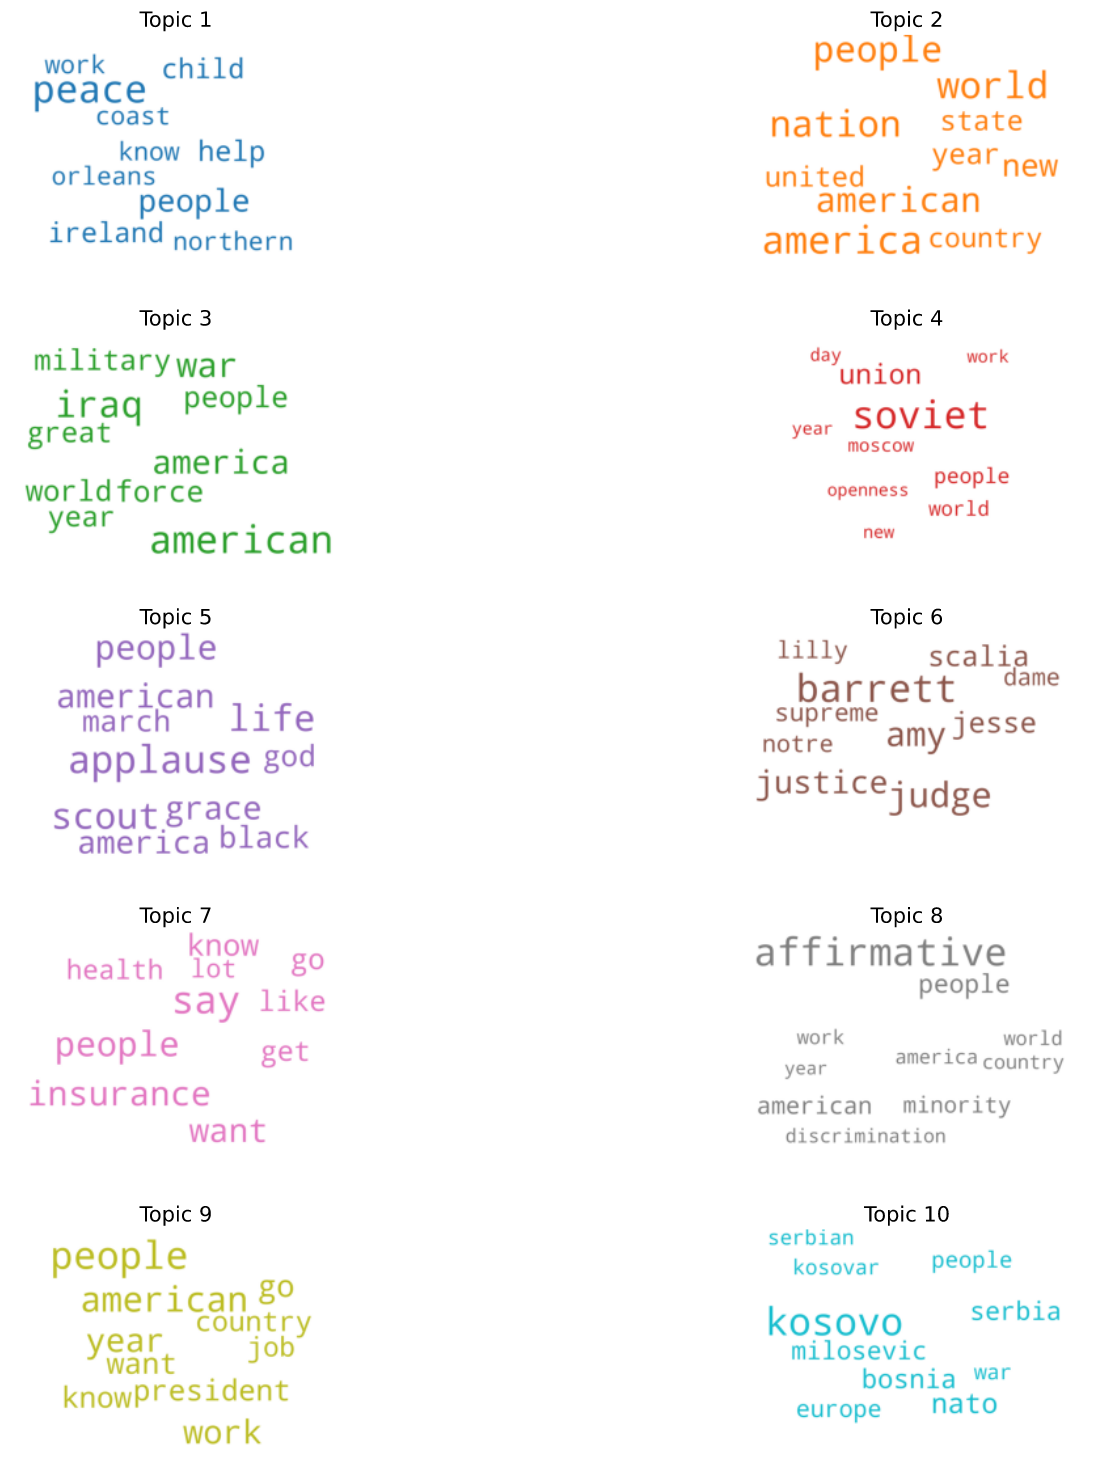
\includegraphics[width=\textwidth]
		{figures/speechestopicmodel.png}}
	\caption{\label{fig:my-label5} Word Clouds of LDA Topic Models for presidential speeches}
\end{figure}

\begin{figure}[!htb]
	\center{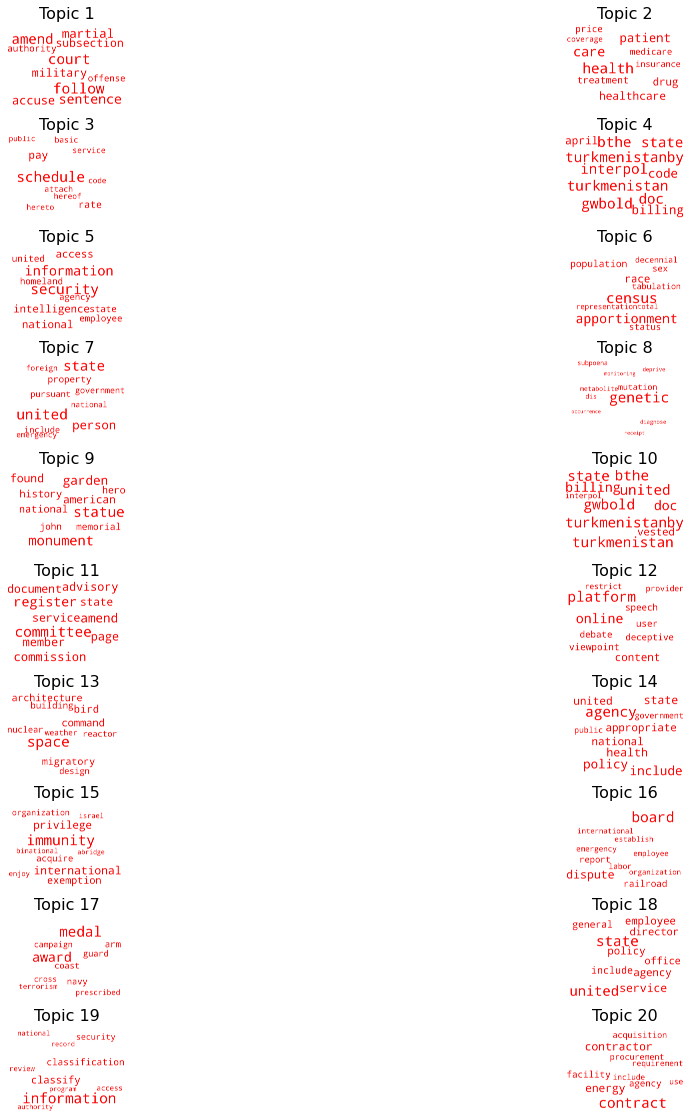
\includegraphics[width=\textwidth]
		{figures/execorderstopics.png}}
	\caption{\label{fig:my-label6} Word Clouds of LDA Topic Models for executive orders}
\end{figure}
}
\end{document}
